% !TEX root = ../main.tex
% --+ 10.21 CEBAF +----------------------------------------------
\begin{frame}{Continuous Electron Beam Accelerator Facility (CEBAF)}
    \label{10.21::cebaf}

    \begin{itemize}
        \item
            \ef{CEBAF} is the linear particle accelerator housed at \ef{JLab} (Jefferson Lab).

        \item
            By recirculating an $e^-$ beam in two 1.4-km-long linear accelerators, the accelerator reaches a \ef{beam energy of $\sim12$ GeV}.

        \item
            Designed for high-energy $e^-$ experiments, CEBAF is ideal for DIS studies.
    \end{itemize}
    \begin{center}
        \begin{figure}[t]
            \centering{
                \fbox{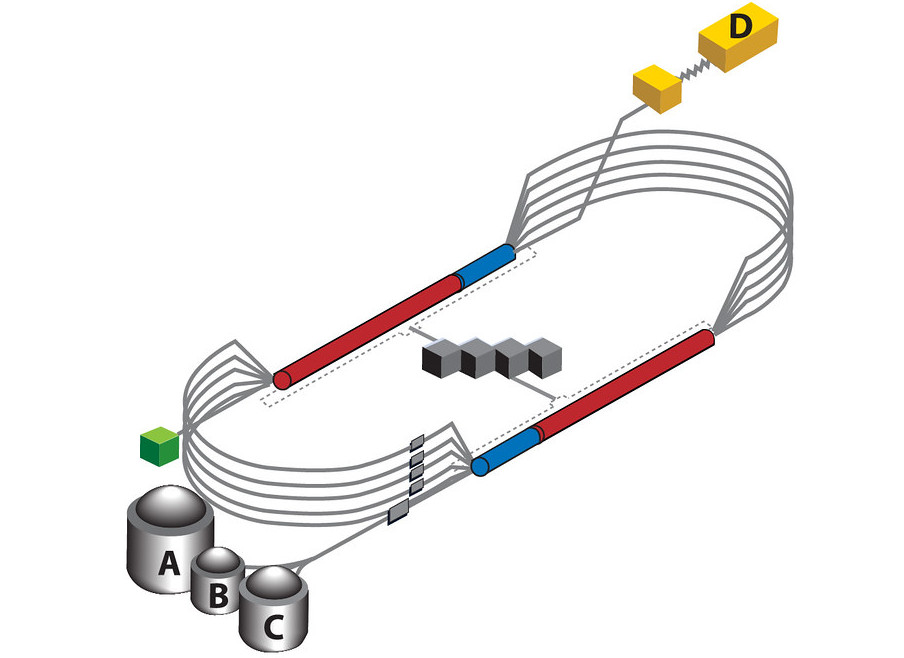
\includegraphics[width=0.5\textwidth]{21cebaf.jpg}}
            }

            \scriptsize{\textit{
                CEBAF diagram.
                The two linear accelerators and experiment halls A to D are pictured.
            }}
        \end{figure}
    \end{center}
\end{frame}

\begin{frame}{CEBAF Large Acceptance Spectrometer for 12 GeV (CLAS12)}
    \label{10.22::clas}

    \begin{itemize}
        \item
            \ef{CLAS12} is the main particle detector at Hall B.

        \item
            The spectrometer is based on two magnets: a solenoid and a 5 T torus.

        \item
            The CLAS12 Forward Detector (FD) has a \ef{polar coverage from $5\degree$ to $35\degree$} and \ef{full azimuthal coverage}.
    \end{itemize}

    \vspace{-12pt}
    \begin{columns}[onlytextwidth,T]

    \begin{column}{.59\linewidth}
        \begin{center}
            \begin{figure}[t]
                \centering{
                    \fbox{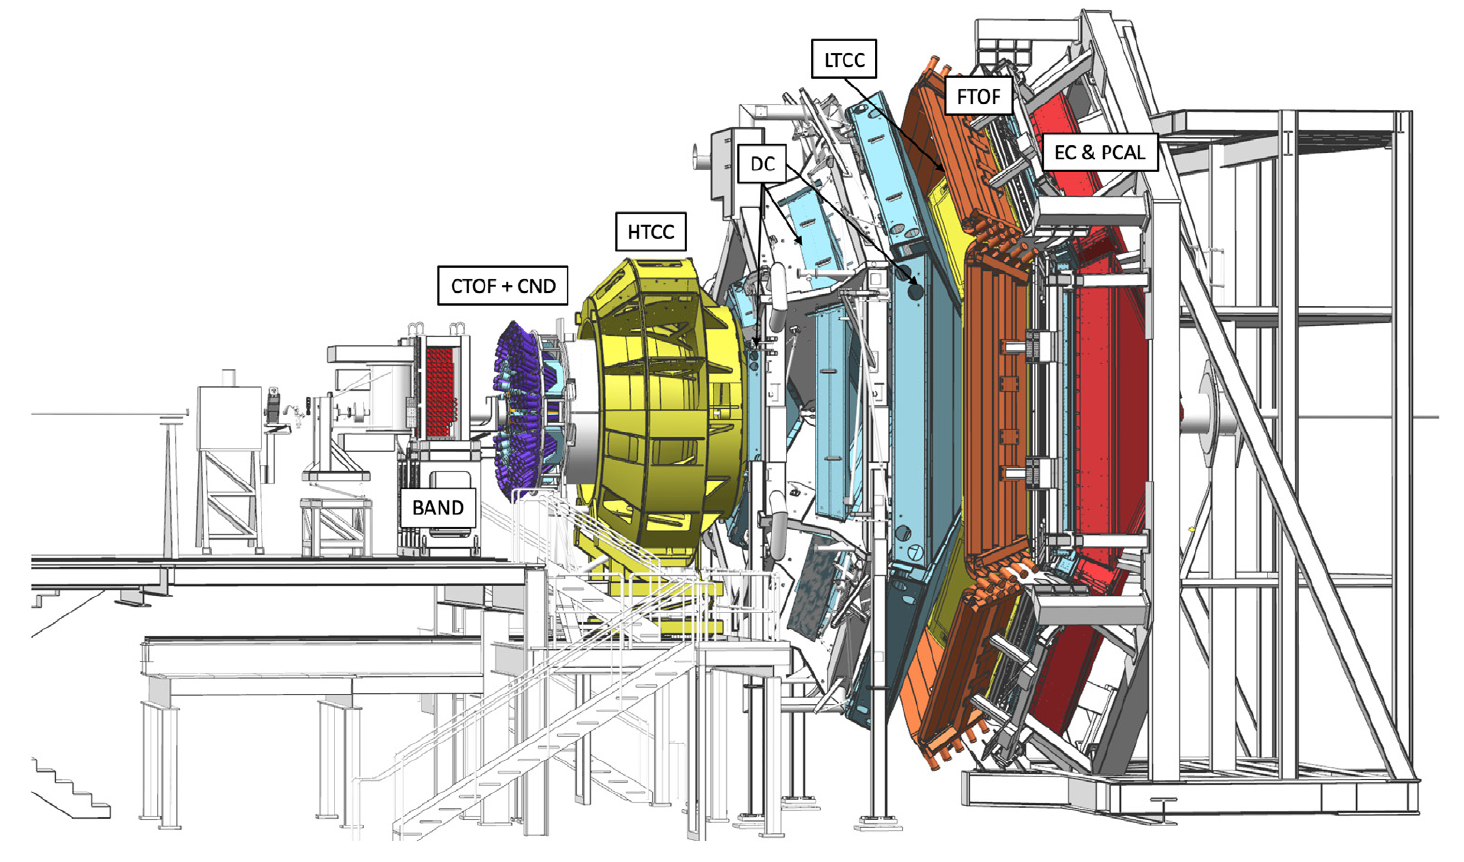
\includegraphics[width=\textwidth]{22clas12.png}}
                }
            \end{figure}
        \end{center}
    \end{column}

    \begin{column}{.39\linewidth}
        \vspace{30pt}
        \scriptsize{\textit{
            CLAS12 diagram.
            \begin{itemize}
                \vspace{6pt}
                \item
                    \ef{BAND}, \ef{CTOF}, and \ef{CND} are not used in this study.
                \vspace{6pt}
                \item
                    \ef{HTCC}, \ef{LTCC}, and \ef{FTOF} are used in particle identification and event time measurement.
                \vspace{6pt}
                \item
                    \ef{EC} and \ef{PCAL} are the FD calorimeters.
                \vspace{6pt}
                \item
                    \ef{DC} and \ef{FMT} (not pictured) are particle trackers.
            \end{itemize}
        }}
    \end{column}

    \end{columns}
\end{frame}

